\documentclass[a4paper,10pt,twocolumn]{ltjsarticle}

% =========================
% 基本パッケージと版面設定
% =========================
\usepackage[top=25mm,bottom=25mm,left=25mm,right=25mm]{geometry}
\setlength{\parindent}{1\zw}
\setlength{\parskip}{0pt}

% =========================
% フォント(LuaTeX-ja)
% =========================
\usepackage{fontspec}
\usepackage{luatexja,luatexja-fontspec}
\defaultfontfeatures{Ligatures=TeX}
\IfFontExistsTF{Times New Roman}{%
  \setmainfont{Times New Roman}%
}{%
  \setmainfont{TeX Gyre Termes}%
}
\IfFontExistsTF{HaranoAjiMincho}{%
  \setmainjfont{HaranoAjiMincho}[BoldFont=HaranoAjiMincho-Bold]%
}{%
  \IfFontExistsTF{Hiragino Mincho ProN W3}{%
    \setmainjfont{Hiragino Mincho ProN W3}[BoldFont=Hiragino Mincho ProN W6]%
  }{%
    \setmainjfont{IPAexMincho}[BoldFont=IPAexMincho]%
  }%
}
\ltjsetparameter{kanjiskip=0pt,xkanjiskip=0pt} % 行長の伸縮を抑止

% =========================
% 数式・記号
% =========================
\usepackage{amsmath,amssymb,bm}

% =========================
% 参考文献(数値引用)
% =========================
\usepackage{cite}
% 全角かっこで [1] → [1] にしたい場合(任意)
\renewcommand\citeleft{[}
\renewcommand\citeright{]}

% 参考文献の行間・段落間隔の調整
\usepackage{etoolbox}
\makeatletter
\pretocmd{\thebibliography}{%
  \setlength{\itemsep}{0pt}%
  \setlength{\parskip}{0pt}%
}{}{}
% 参考文献ラベル(本文末の見出し側)も全角に(任意)
\renewcommand\@biblabel[1]{[#1]}
\makeatother

% =========================
% 表・単位
% =========================
\usepackage{booktabs}
\usepackage{siunitx}
\sisetup{detect-all}
\usepackage{threeparttable}

% =========================
% 図・画像
% =========================
\usepackage{graphicx}
\graphicspath{{img/}}

% =========================
% キャプション(体裁を一括指定)
% =========================
\usepackage{caption}
\captionsetup{font=small,labelfont=bf}
% 英文風表記に統一
\renewcommand{\figurename}{Fig.}
\renewcommand{\tablename}{Table~}
% 区切り “Fig. 2. …”, “Table 1. …”
\captionsetup[figure]{labelsep=period}
\captionsetup[table]{labelsep=period}

% フロート周りの間隔
\setlength{\textfloatsep}{.5\baselineskip}
\setlength{\intextsep}{.5\baselineskip}
\setlength{\abovecaptionskip}{.25\baselineskip}
\setlength{\belowcaptionskip}{0pt}

% =========================
% 見出し(グリッドを維持)
% =========================
\usepackage{titlesec}
\titleformat{\section}{\bfseries\normalsize}{\thesection}{.5\zw}{}
\titlespacing{\section}{0pt}{0pt}{0pt}
\titleformat{\subsection}{\bfseries\normalsize}{\thesubsection}{.5\zw}{}
\titlespacing{\subsection}{0pt}{0pt}{0pt}

% =========================
% ページスタイル
% =========================
\usepackage{fancyhdr} % ← \fancypagestyle より前に読み込む
\pagestyle{empty}

% --- Footer: さらに1cm上/線は3倍太く ---
\fancypagestyle{firstpage}{%
  \fancyhf{}%
  \renewcommand{\headrulewidth}{0pt}%
  \renewcommand{\footrulewidth}{2pt}% 線の太さは既定どおり
  \renewcommand{\footruleskip}{.3\normalbaselineskip}% ★ 既定に固定:線の位置を動かさない
  \fancyfoot[L]{%
    % ★ 文字だけ3mm下げる. 高さ/深さを0に潰すのでレイアウトに影響しない
    \smash{\raisebox{1mm}{%
      Ichiro FUNTAI: TEL: 075-351-2318\quad E-mail: office@sptj.jp\ (ただし1ページ目のみ)
    }}%
  }%
}

% =========================
% 2段ヘッダ用ヘルパ(mm単位)
% =========================
% 題目用の日本語ボールドフォント(\TitleJ 定義)
\IfFontExistsTF{HaranoAjiMincho-Bold}{%
  \newjfontfamily\TitleJ{HaranoAjiMincho-Bold}%
}{%
  \IfFontExistsTF{Hiragino Mincho ProN W6}{%
    \newjfontfamily\TitleJ{Hiragino Mincho ProN W6}%
  }{%
    \newjfontfamily\TitleJ{IPAexMincho}[FakeBold=2]%
  }%
}

% 研究報告:1mm左・1mm下(= 右オフセット 3mm→2mm, 上げ量 1mm→0mm)
\newcommand{\ReportType}[1]{%
  \noindent\hspace*{8\zw}\hspace*{3mm}\raisebox{1.5mm}[0pt][0pt]{#1}\par}

% 題目:1mm下(= 上げ量 1mm→0mm)
\newcommand{\TitleLine}[1]{%
  \begin{center}%
    \hspace*{0mm}\raisebox{2mm}[0pt][0pt]{\TitleJ\bfseries\fontsize{14pt}{16pt}\selectfont #1}%
  \end{center}}

% 著者行:2mm上・2mm左(= \raisebox に +2mm, 右寄せボックス幅を 2mm 縮める)
\newcommand{\AuthorsLine}[1]{%
  \noindent\raisebox{\dimexpr\baselineskip -1.3mm\relax}[0pt][0pt]{%
    \makebox[\dimexpr \textwidth - 2\zw + 0.8mm\relax][r]{#1}}\par}

% =========================
% 参照マクロ
% =========================
\newcommand{\refSec}[1]{Section~\ref{#1}}
\newcommand{\refFig}[1]{Fig.~\ref{#1}}
\newcommand{\refTab}[1]{Table~\ref{#1}}
\newcommand{\refEq}[1]{Eq.~\eqref{#1}}

% =========================
% グリッド:1段=22字(=22zw) × 48行
% =========================
\newlength{\GridBase}
\setlength{\GridBase}{14.625pt} % ≈ 247mm/48
\newlength{\ReduceCenterBy}     % 中央を狭める量(最大10mm)
\setlength{\ReduceCenterBy}{10mm}

\AtBeginDocument{%
  \fontsize{10pt}{\GridBase}\selectfont
  \setlength{\baselineskip}{\GridBase}%
  \setlength{\textheight}{48\baselineskip}%
  % 列幅=22zw を優先:columnsep = textwidth - 44zw から 10mm 減らし, 負なら0に飽和
  \setlength{\columnsep}{\dimexpr \textwidth - 44\zw - \ReduceCenterBy\relax}%
  \ifdim\columnsep<0pt \setlength{\columnsep}{0pt}\fi
  % 「文章は全体的に1mm上へ」→ 1行目基準を1mm上に
  \setlength{\topskip}{\dimexpr \baselineskip + \GridBase - 1mm\relax}%
  \setlength{\textheight}{\dimexpr 48\baselineskip - 9mm\relax}%
}

% =========================
% 出力フック(1ページ目以外の行数拡張)
% =========================
\usepackage{atbegshi}
\AtBeginShipoutNext{%
  % 以後のページにだけ適用(1ページ目は shipout 済みなので不変)
  \global\addtolength{\topskip}{-2\baselineskip}%   1行目基準を2行ぶん上へ
  \global\addtolength{\textheight}{-1\baselineskip}% 本文行数を合計5行ぶん拡張(上2 + 下3)
}
%%%%%%%%%%%%%%%%%%%%%%%%%%%%%%%%%%%%%%%%%%%%%%%%%%%%%%%%%%%%%%%%%%%%%%%%%%%%%%%%%%%%%%%%%%%%%%%%
\begin{document}
\thispagestyle{firstpage}
\twocolumn[{
      \vspace*{\GridBase}
      \ReportType{「研究報告」*10ポイント以上}
      \vspace{.5\baselineskip}
      \TitleLine{講演要旨集執筆要綱(14\,ポイント)}
      \vspace{.5\baselineskip}
      \AuthorsLine{粉体工学会事務局\quad ○粉体 一郎,粉体 二郎,粉体 三郎}
      \vspace{.5\baselineskip}
      \vspace*{-7mm}
    }]
\AtBeginShipoutNext{%
  \global\addtolength{\topskip}{-2\baselineskip}
  \global\addtolength{\textheight}{2\baselineskip}
}
%%%%%%%%%%%%%%%%%%%%%%%%%%%%%%%%%%%%%%%%%%%%%%%%%%%%%%%%%%%%%%%%%%%%%%%%%%%%%%%%%%%%%%%%%%%%%%%%
\section{緒言}
講演要旨の執筆にあたり,以下の各事項に準拠して下さい. 講演要旨は,講演1件に対して図表を含めてA4サイズ,2ページです. 書式は,2段組み,1段当たり22字×48行を基準とします. マージンは,上下左右それぞれ25\,mmとして下さい. フォントは,標準的なものとして,日本語は明朝体,英文は Times New Roman を推奨しますが,他のフォントでも結構です. 文字の大きさは10ポイント以上,英数字はすべて半角にして下さい. 文字数,文字間隔,行数等には厳密にはこだわりませんが,読みやすさに配慮して下さい. 図表は白黒・カラーのどちらでも構いませんが,要旨集は白黒で印刷します. 印刷時に鮮明になるように留意して下さい. また図表中の説明や記号などが小さくなりすぎないように注意して下さい. 数式などはイタリック体で表記し,上付き/下付きの字が小さくなりすぎないようにして下さい. 原則2ページを越す場合には事務局(\texttt{office@sptj.jp})までご相談ください.


\begin{center}
  \vspace*{.25\baselineskip} % ★ minipage先頭で必ず効く
  \fbox{\rule{0pt}{30mm}\rule{23\zw}{0pt}}
  \captionof{figure}{, 図1|キャプション}
\end{center}

\par\addvspace{.75\baselineskip}


\section{原稿の書き方}
\subsection{講演情報}
この見本のように,原稿1ページ目の左上部には講演番号を入れるための余白として第1行目の左マージンから8文字分を空白としてあけ,「研究報告」「技術報告」「技術資料」等の種別を記入して下さい. 1行あけて第2行目中央に,講演題目を14ポイントで記入して下さい. 講演題目からさらに1行あけて第3行目に,発表者の所属,氏名を右寄せで記入して下さい. 講演者には必ず○印を付けて下さい. 連名などで1行に書ききれない場合は2行以上でも結構です. また原稿1ページ目下欄外に,発表者のローマ字表記名,連絡先の電話番号,電子メールアドレスを1行で記入して下さい. ローマ字表記名については,氏(頭文字のみ大文字,以下小文字),姓(すべて大文字)の順で記入して下さい. ただし1ページ目のみです.

\subsection{本文}
本文は,発表者の所属,氏名から1行あけて書き始めて下さい. 2ページ目以降は1行目から書いて下さい. また偶数ページ/奇数ページにかかわらず,どのページも印字部分が用紙の中央になるように設定して下さい.

\par\addvspace{.75\baselineskip}


\section{講演要旨の提出}
講演要旨は,関連行事の要旨提出URLよりご提出ください. ファイルサイズは3\,MB以下の,pdfまたはwordファイル(拡張子:pdf,docまたはdocx)のみ受付可能です. ファイルのアップロードには,受付番号とパスワードが必要です. 締切までの期間内は,講演要旨の投稿を繰り返すことができます.

\par\addvspace{.75\baselineskip}


%%%%%%%%%%%%%%%%%%%%%%%%%%%%%%%%%%%%%%%%%%%%%%%%%%%%%%%%%%%%%%%%%%%%%%%%%%%%%%%%%%%%%%%%%%%%%%%%
\section{DEMにおけるVoigtモデル}
離散要素法(DEM)では,接触中の粒子対 $i$–$j$ を法線方向と接線方向に直交分解し,それぞれを線形ばねとダッシュポットを並列接続したVoigt要素で近似する \cite{Cundall1979}.圧縮を正,接触法線単位ベクトルを $\bm n$ とする.
粒子–粒子接触におけるVoigtモデル(ばね–ダッシュポット)の構成要素と向きを \refFig{fig:voigt} に示す.

\noindent\begin{minipage}{\columnwidth}\centering
  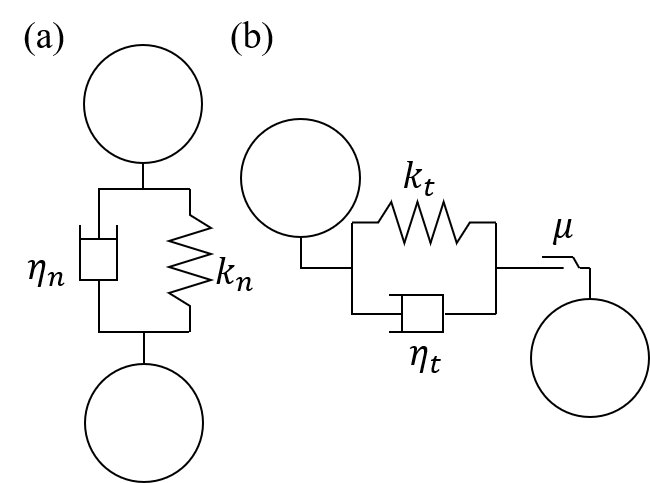
\includegraphics[width=\columnwidth]{voigt_model}
  \captionof{figure}{Schematic of particle–particle contact in the Voigt model: (a) normal interaction, (b) tangential interaction.}
  \label{fig:voigt}
\end{minipage}

\subsection{法線方向}
重なり$\delta_n$ と法線相対速度 $v_n=\bigl(\bm v_{ij}\cdot\bm n\bigr)$ から,法線力は
\begin{align}
  \bm F_n
  = \Bigl(k_n\,\delta_n - \gamma_n\, v_n \Bigr)\,\bm n ,
  \label{eq:Fn}
\end{align}
で与える.$k_n$ は法線ばね定数,$\gamma_n$ は法線減衰係数である.

\subsection{接線方向}
Cundall--Strack に従い \cite{Cundall1979},接触座標系で積分した接線ばね伸び $\bm\xi_t$ を用いる.接線相対速度は
\begin{align}
  \bm v_t & = \bm v_{ij} - (\bm v_{ij}\!\cdot\!\bm n)\,\bm n
  - R_i\,(\bm\omega_i\!\times\!\bm n)
  - R_j\,(\bm\omega_j\!\times\!\bm n),
\end{align}
で与える.接線力の試行値と最終値は
\begin{align}
  \bm F_t^\ast & = -k_t\,\bm\xi_t - \gamma_t\,\bm v_t,                          \\
  \bm F_t      & = -\,\min\!\Bigl(\,\|\bm F_t^\ast\|,\ \mu\,|\bm F_n|\,\Bigr)\,
  \frac{\bm F_t^\ast}{\|\bm F_t^\ast\|},
  \label{eq:Ft_min}
\end{align}
で与える. ここで$\mu$ はクーロン摩擦係数である.

\subsection{転がり摩擦}
球粒子は接線摩擦のみでは過大回転しやすいため,接触点まわりの転がり抵抗モーメント $\bm\tau_r$ を導入して回転を抑制する \cite{Iwashita1998}.有効半径は $R^\ast=R_iR_j/(R_i+R_j)$,相対角速度は $\bm\omega_\mathrm{rel}=\bm\omega_i-\bm\omega_j$ と表される.
回転ばね角度履歴 $\bm\theta_r$ を用いて
\begin{align}
  \bm\tau_r^\ast & = -k_r\,\bm\theta_r - \gamma_r\,\bm\omega_\mathrm{rel},                    \\
  \bm\tau_r      & = -\,\min\!\Bigl(\,\|\bm\tau_r^\ast\|,\ \mu_r\,|\bm F_n|\,R^\ast\,\Bigr)\,
  \frac{\bm\tau_r^\ast}{\|\bm\tau_r^\ast\|}.
  \label{eq:rr_min}
\end{align}
静的・動的の転がり抵抗を統一的に表現でき,安息角や回転率の再現性が高い.

\section{時間積分}
本研究では,粒子の並進・回転運動をシンプレクティック・オイラー法で時間積分する.
粒子 $i$ の質量を $m_i$,慣性モーメントを $I_i$,位置を $\bm r_i$,速度を $\bm v_i$,
角速度を $\bm\omega_i$,回転角(姿勢パラメータ)を $\bm\theta_i$,作用する合力・合モーメントを
それぞれ $\bm F_i,\ \bm\tau_i$ とすると,運動方程式は
\begin{align}
  m_i\,\dot{\bm v}_i     & = \bm F_i,      &
  \dot{\bm r}_i          & = \bm v_i,      &
  I_i\,\dot{\bm\omega}_i & = \bm\tau_i,    &
  \dot{\bm\theta}_i      & = \bm\omega_i .
\end{align}
シンプレクティック・オイラー法による更新は,まず速度・角速度を更新し,その新しい値で位置・角度を更新する.
\begin{align}
  \bm v_i^{n+1}       & = \bm v_i^{n}      + \Delta t\,\frac{\bm F_i^{\,n}}{m_i},   \\
  \bm\omega_i^{n+1}   & = \bm\omega_i^{n}  + \Delta t\,\frac{\bm\tau_i^{\,n}}{I_i}, \\
  \bm r_i^{n+1}       & = \bm r_i^{n}      + \Delta t\,\bm v_i^{\,n+1},             \\
  \bm\theta_i^{\,n+1} & = \bm\theta_i^{\,n}+ \Delta t\,\bm\omega_i^{\,n+1}.
\end{align}

\section{シミュレーション条件}
本研究のシミュレーションに用いた主要パラメータを \refTab{tab:params-compact} に示す.

\noindent\begin{minipage}{\columnwidth}\centering
  \begingroup
  \setlength{\tabcolsep}{3pt}
  \footnotesize
  \begin{threeparttable}
    \captionof{table}{Simulation parameters.}
    \label{tab:params-compact}
    \begin{tabular}{@{}llSS@{}}
      \toprule
      Symbol     & Parameter                  & {Value} & {Units}                              \\
      \midrule
      $\rho$     & density                    & 2.50e3  & \si{\kilogram\per\meter\cubed}       \\
      $R$        & particle radius (all same) & 1.00e-3 & \si{\meter}                          \\
      \midrule
      $k_n$      & normal spring              & 1.00e4  & \si{\newton\per\meter}               \\
      $\gamma_n$ & normal dashpot             & 1.00e-3 & \si{\kilogram\per\second}            \\
      $k_t$      & tangential spring          & 6.00e3  & \si{\newton\per\meter}               \\
      $\gamma_t$ & tangential dashpot         & 1.00e-3 & \si{\kilogram\per\second}            \\
      $\mu$      & Coulomb friction           & 5.00e-1 & {}                                   \\
      \midrule
      $\eta_r$   & viscous rolling resistance & 2.00e-8 & \si{\newton\meter\second}            \\
      $k_r$      & rotational spring          & 1.00e-6 & \si{\newton\meter\per\radian}        \\
      $\gamma_r$ & rotational dashpot         & 1.00e-8 & \si{\newton\meter\second\per\radian} \\
      $\mu_r$    & rolling friction           & 5.00e-2 & {}                                   \\
      \bottomrule
    \end{tabular}
  \end{threeparttable}
  \endgroup
\end{minipage}


%%%%%%%%%%%%%%%%%%%%%%%%%%%%%%%%%%%%%%%%%%%%%%%%%%%%%%%%%%%%%%%%%%%%%%%%%%%%%%%%%%%%%%%%%%%%%%%%
\par\addvspace{.75\baselineskip}
% 参考文献
\begin{thebibliography}{99}
  \bibitem{Cundall1979}
  P. A. Cundall and O. D. L. Strack, Géotechnique, \textbf{29} (1979) 47--65.
  \bibitem{Iwashita1998}
  K. Iwashita and M. Oda, Journal of Engineering Mechanics (ASCE), \textbf{124} (1998) 285--292.
\end{thebibliography}
%%%%%%%%%%%%%%%%%%%%%%%%%%%%%%%%%%%%%%%%%%%%%%%%%%%%%%%%%%%%%%%%%%%%%%%%%%%%%%%%%%%%%%%%%%%%%%%%
\end{document}
